\section{Cross-Domain Results}\label{sec:cross_results}

Some of the variations below include a Canny edge detector as a preprocessing
step. The parameter $\sigma$ determines the size of the Gaussian kernel used by
the Canny algorithm. A value of $\sigma = 1.5$ was determined to be appropriate
for the image dataset used in the benchmark. Values larger than $\sigma = 2$
tend not to detect any edges, while smaller values produced more "false" edges
resulting from noise in the images.

The SEGMENT preprocessing step could unfortunately not use the same $1024
\times 768$ pixel images as inputs as the other preprocessors, because the
implementation provided by Arbelaez et al.\ \autocite{arbelaez_contour_2011}
could not be run on any machine available due to extreme memory requirements.
Therefore, the images in the database are rescaled to $320 \times 240$ pixels
for the evaluation of this algorithm. This might lead to loss of small features
    and puts limits on some parameters like the grid size $G$.

All pipeline variants utilize the FDCT to extract curve information. The number
of scales and the number of angles at the coarsest scale will be called $N_s$
and $N_{\theta}$ respectively. Based on experimentation and other publications
using the curvelet transform \autocite{mandal_curvelet_2009}
\autocite{guha_curvelet_2010}, 4 scales and 12 angles are used in almost all
cases, since larger values did not consistently lead to better results. The
size of the codebook is set at 1000 visual words, as values beyond that did
not show improvements in evaluations performed by Nowak at al.\
\autocite{nowak_sampling_2006}. Eitz et al.\ \autocite{eitz_sketch-based_2011}
reported similar optimal values of 500 to 1000 visual words and attributed the
low number to the sparsity of edge-like features in sketches.

Throughout the correlation coefficient graphs in the following sections, the
results obtained by Eitz et al.\ \autocite{eitz_sketch-based_2011} for the HoG,
Spark and SHoG descriptors are included.

The first two sections present the resulting mean $\tau_B$ values obtained
using the rank correlation method described above, grouped by preprocessing
steps and sampling method. Afterwards, the influence of parameter variations
and the distribution of results within selected pipelines are examined.

\subsection{Global Features}

The processing steps applied to the database images and the query images in the
pipelines based on global features are almost identical, with the exception of
the CANNY, SOBEL and SEGMENT steps for the database images. The curvelet
responses are averaged on a grid and the features are ranked using the $L_2$
and the COS distance measures.

\paragraph{LUMA+MEAN}

The most straightforward combination of processing steps consists of a LUMA
input image, on which the means of $G \times G$ grid cells is computed for each
scale and angle (Figure \ref{fig:pipeline_global_luma_mean}).  Varying $G$
determines the feature size that can be encoded best. Setting $G=12$ seems to
yield the best correlation, although the advantage over $G=8$ and $G=16$ is
below $0.01$. The distance measure COS outperforms the $L_2$ measure (Table
\ref{tab:results_global_luma_mean}). A possible explanation would be that the
COS measure normalizes the magnitude of the feature vector as discussed in
\ref{sec:anatomy_ranking_distance_euclidean}.

\begin{figure}[h]
    \centering
    \begin{tikzpicture}[font=\tiny]
    \matrix[node grid] {
        \node [document node] (dbimg) {$I_{db}$}; &
        \node [operation node] (dbluma) {LUMA}; &
        \node [operation node] (dbcurvelet) {FDCT}; &
        \node [operation node] (dbmean) {MEAN}; \\
        \node [document node] (qimg) {$I_q$}; &
        \node [operation node] (qluma) {LUMA}; &
        \node [operation node] (qcurvelet) {FDCT}; &
        \node [operation node] (qmean) {MEAN}; \\
    };

    \node [operation node, split node=2, right=3ex of $(dbmean.east)!0.5!(qmean.east)$] (dist) {$L_2$ \nodepart{two} COS};
    \node [document node, right=of dist] (result) {distances};

    \node [parameter node, above=of dbcurvelet] (dbcurveletparam) {$(N_s, N_{\theta})$};
    \node [parameter node, above=of dbmean] (dbmeanparam) {$G$};
    \node [parameter node, below=of qcurvelet] (qcurveletparam) {$(N_s, N_{\theta})$};
    \node [parameter node, below=of qmean] (qmeanparam) {$G$};

    \path [parameter connector] (dbcurveletparam) -- (dbcurvelet);
    \path [parameter connector] (dbmeanparam) -- (dbmean);
    \path [parameter connector] (qcurveletparam) -- (qcurvelet);
    \path [parameter connector] (qmeanparam) -- (qmean);

    { [start chain=going right, every join/.style={connector}]
        \chainin (dbimg);
        \chainin (dbluma) [join];
        \chainin (dbcurvelet) [join];
        \chainin (dbmean) [join];
        \chainin (dist) [join=with dbmean.east by hvh connector top];
    }
    { [start chain=going right, every join/.style={connector}]
        \chainin (qimg);
        \chainin (qluma) [join];
        \chainin (qcurvelet) [join];
        \chainin (qmean) [join];
        \chainin (dist) [join=with qmean.east by hvh connector bottom];
        \chainin (result) [join];
    }
\end{tikzpicture}

    \caption[Global LUMA+MEAN Pipelines]{
        Global LUMA+MEAN Pipelines
    }
    \label{fig:pipeline_global_luma_mean}
\end{figure}

\begin{table}[h]
    \centering
    \pgfplotstableread[]{results/g_luma_mean_1.csv}\resultsglumamean

\plottablexbars{scales,angles,gridsize,metric}{\resultsglumamean}

%\newcommand{\plotxbars}[#1]{%
%\begin{tikzpicture} %[trim axis left,trim axis right]
    %\begin{axis}[
        %hbarplot,
        %width=6cm,
        %%xcomb,
        %%small,
        %%y=-\baselineskip,
        %%scale only axis,
        %%enlarge y limits={abs=0.45},
        %%ytick=\empty,
        %%axis x line*=bottom,
        %%axis y line*=left,
        %%yticklabels from table={\resultsglumamean}{Description},
        %]
        %\addplot table[x=MeanCorrelation, y expr=\coordindex] {#1};
        %\addreferenceplot;
    %\end{axis}
%\end{tikzpicture}%
%}

%\newcommand{\tablexbars}[1]{
    %\pgfplotstabletypeset[columns={scales,angles,grid_size,metric,graph},
      %% Booktabs rules
      %every head row/.style={after row=\midrule},
      %every last row/.style={after row=[3ex]},
      %% Set header name
      %columns/scales/.style={string type,column name=$N_s$},
      %columns/angles/.style={string type,column name=$N_{\theta}$},
      %columns/grid_size/.style={string type,column name=$G$},
      %columns/canny_sigma/.style={string type,column name=$\sigma$},
      %columns/metric/.style={string type,column name=Metric},
      %columns/graph/.style={
        %column name={},
        %assign cell content/.code={% use \multirow for Z column:
        %\ifnum\pgfplotstablerow=0
        %\pgfkeyssetvalue{/pgfplots/table/@cell content}
        %{\multirow{\pgfplotstablegetrowsof{\resultsglumamean}\pgfplotsretval}{5cm}{\theplot}}%
        %\else
        %\pgfkeyssetvalue{/pgfplots/table/@cell content}{}%
        %\fi
        %}
      %},
    %]{\resultsglumamean}
%}

    \caption[Global LUMA+MEAN Results]{
        Global LUMA+MEAN Results
    }
    \label{tab:results_global_luma_mean}
\end{table}

\paragraph{CANNY+MEAN}

In addition to reading the images like in the previous LUMA+MEAN configuration,
this pipeline applies a CANNY processing step to the database images in an
attempt to bring the query and database image domains closer together (Figure
\ref{fig:pipeline_global_luma_canny_mean}). Again, the COS distance measure
produces the best rankings (Table~\ref{tab:results_global_luma_canny_mean}).
Surprisingly, the Canny edge detector does not lead to increased performance in
comparison to plain the LUMA preprocessing step.

\begin{figure}[h]
    \centering
    \begin{tikzpicture}[font=\tiny]
    \matrix[node grid] {
        \node [document node] (dbimg) {$I_{db}$}; &
        \node [operation node] (dbluma) {LUMA}; &
        \node [operation node] (dbcanny) {CANNY};  &
        \node [operation node] (dbcurvelet) {FDCT}; &
        \node [operation node] (dbmean) {MEAN}; \\
        \node [document node] (qimg) {$I_q$}; &
        \node [operation node] (qluma) {LUMA}; &&
        \node [operation node] (qcurvelet) {FDCT}; &
        \node [operation node] (qmean) {MEAN}; \\
    };

    \node [operation node, split node=2, right=3ex of $(dbmean.east)!0.5!(qmean.east)$] (dist) {$L_2$ \nodepart{two} COS};
    \node [document node, right=of dist] (result) {distances};

    \node [parameter node, above=of dbcanny] (dbcannyparam) {$\sigma$};
    \node [parameter node, above=of dbcurvelet] (dbcurveletparam) {$(N_s, N_{\theta})$};
    \node [parameter node, above=of dbmean] (dbmeanparam) {$G$};
    \node [parameter node, below=of qcurvelet] (qcurveletparam) {$(N_s, N_{\theta})$};
    \node [parameter node, below=of qmean] (qmeanparam) {$G$};

    \path [parameter connector] (dbcannyparam) -- (dbcanny);
    \path [parameter connector] (dbcurveletparam) -- (dbcurvelet);
    \path [parameter connector] (dbmeanparam) -- (dbmean);
    \path [parameter connector] (qcurveletparam) -- (qcurvelet);
    \path [parameter connector] (qmeanparam) -- (qmean);

    { [start chain=going right, every join/.style={connector}]
        \chainin (dbimg);
        \chainin (dbluma) [join];
        \chainin (dbcanny) [join];
        \chainin (dbcurvelet) [join];
        \chainin (dbmean) [join];
        \chainin (dist) [join=with dbmean.east by hvh connector top];
    }
    { [start chain=going right, every join/.style={connector}]
        \chainin (qimg);
        \chainin (qluma) [join];
        \chainin (qcurvelet) [join];
        \chainin (qmean) [join];
        \chainin (dist) [join=with qmean.east by hvh connector bottom];
        \chainin (result) [join];
    }
\end{tikzpicture}

    \caption[Global CANNY+MEAN Pipelines]{
        Global CANNY+MEAN Pipelines
    }
    \label{fig:pipeline_global_luma_canny_mean}
\end{figure}

\begin{table}[h]
    \centering
    \pgfplotstableread[]{results/g_luma_canny_mean_1.csv}\resultsglumacannymean
\begin{tikzpicture}
    \begin{axis}[
        hbarplot,
        yticklabels from table={\resultsglumacannymean}{Description},
        ]
        \addplot table[x=MeanCorrelation, y expr=\coordindex] {\resultsglumacannymean};
        \addreferenceplot;
    \end{axis}
\end{tikzpicture}

    \caption[Global CANNY+MEAN Results]{
        Global CANNY+MEAN Results
    }
    \label{tab:results_global_luma_canny_mean}
\end{table}

\paragraph{SOBEL+MEAN}

The SOBEL step used in this variant also attempts to bring the database images
into the sketch domain (Figure~\ref{fig:pipeline_global_luma_sobel_mean}). The
results are slightly better than with the CANNY preprocessor
(Table~\ref{tab:results_global_luma_sobel_mean}).

\begin{figure}[h]
    \centering
    \begin{tikzpicture}[font=\tiny]
    \matrix[node grid] {
        \node [document node] (dbimg) {$I_{db}$}; &
        \node [operation node] (dbluma) {LUMA}; &
        \node [operation node] (dbcanny) {SOBEL};  &
        \node [operation node] (dbcurvelet) {FDCT}; &
        \node [operation node] (dbmean) {MEAN}; \\
        \node [document node] (qimg) {$I_q$}; &
        \node [operation node] (qluma) {LUMA}; &&
        \node [operation node] (qcurvelet) {FDCT}; &
        \node [operation node] (qmean) {MEAN}; \\
    };

    \node [operation node, split node=2, right=3ex of $(dbmean.east)!0.5!(qmean.east)$] (dist) {$L_2$ \nodepart{two} COS};
    \node [document node, right=of dist] (result) {distances};

    { [start chain=going right, every join/.style={connector}]
        \chainin (dbimg);
        \chainin (dbluma) [join];
        \chainin (dbcanny) [join];
        \chainin (dbcurvelet) [join];
        \chainin (dbmean) [join];
        \chainin (dist) [join=with dbmean.east by hvh connector top];
    }
    { [start chain=going right, every join/.style={connector}]
        \chainin (qimg);
        \chainin (qluma) [join];
        \chainin (qcurvelet) [join];
        \chainin (qmean) [join];
        \chainin (dist) [join=with qmean.east by hvh connector bottom];
        \chainin (result) [join];
    }
\end{tikzpicture}

    \caption[Global SOBEL+MEAN Pipelines]{
        Global SOBEL+MEAN Pipelines
    }
    \label{fig:pipeline_global_luma_sobel_mean}
\end{figure}

\begin{table}[h]
    \centering
    \pgfplotstableread[]{results/g_luma_sobel_mean_1.csv}\resultsglumasobelmean
\plottablexbars{scales,angles,gridsize,metric}{\resultsglumasobelmean}
%\begin{tikzpicture}
    %\begin{axis}[
        %hbarplot,
        %yticklabels from table={\resultsglumasobelmean}{Description},
        %]
        %\addplot table[x=MeanCorrelation, y expr=\coordindex] {\resultsglumasobelmean};
        %\addreferenceplot;
    %\end{axis}
%\end{tikzpicture}

    \caption[Global SOBEL+MEAN Results]{
        Global SOBEL+MEAN Results
    }
    \label{tab:results_global_luma_sobel_mean}
\end{table}

\paragraph{SEGMENT+MEAN}

With the gPb contour detector in the SEGMENT step to find edges in the database
images (Figure~\ref{fig:pipeline_global_luma_segment_mean}), the $L_2$ distance
metric produces results comparable to the COS metric in the CANNY+MEAN variant
(Table~\ref{tab:results_global_luma_segment_mean}).  Unlike in the other cases,
the COS distance measure performs worse than the $L_2$ metric.

\begin{figure}[h]
    \centering
    \begin{tikzpicture}[font=\tiny]
    \matrix[node grid] {
        \node [document node] (dbimg) {$I_{db}$}; &
        \node [operation node] (dbsegment) {SEGMENT}; &
        \node [operation node] (dbcurvelet) {FDCT}; &
        \node [operation node] (dbmean) {MEAN}; \\
        \node [document node] (qimg) {$I_q$}; &
        \node [operation node] (qluma) {LUMA}; &
        \node [operation node] (qcurvelet) {FDCT}; &
        \node [operation node] (qmean) {MEAN}; \\
    };

    \node [operation node, split node=2, right=3ex of $(dbmean.east)!0.5!(qmean.east)$] (dist) {$L_2$ \nodepart{two} COS};
    \node [document node, right=of dist] (result) {distances};

    { [start chain=going right, every join/.style={connector}]
        \chainin (dbimg);
        \chainin (dbsegment) [join];
        \chainin (dbcurvelet) [join];
        \chainin (dbmean) [join];
        \chainin (dist) [join=with dbmean.east by hvh connector top];
    }
    { [start chain=going right, every join/.style={connector}]
        \chainin (qimg);
        \chainin (qluma) [join];
        \chainin (qcurvelet) [join];
        \chainin (qmean) [join];
        \chainin (dist) [join=with qmean.east by hvh connector bottom];
        \chainin (result) [join];
    }
\end{tikzpicture}

    \caption[Global SEGMENT+MEAN Pipelines]{
        Global SEGMENT+MEAN Pipelines
    }
    \label{fig:pipeline_global_luma_segment_mean}
\end{figure}

\begin{table}[h]
    \centering
    \pgfplotstableread[]{results/g_luma_segment_mean_1.csv}\resultsglumasegmentmean
\plottablexbars{scales,angles,gridsize,metric}{\resultsglumasegmentmean}

    \caption[Global SEGMENT+MEAN Results]{
        Global SEGMENT+MEAN Results
    }
    \label{tab:results_global_luma_segment_mean}
\end{table}

\subsection{Local Features}

The local feature extraction pipelines utilize the same preprocessing steps as
the ones based on global features. The curvelet transform remains unchanged as
well. The the curvelet coefficients are sampled using the PMEANS and PMEANS2
strategy to produce features for local patches. From these feature vectors, a
codebook of size $1000$ is generated and the feature vectors from both the
database images and the query images are quantized 

\paragraph{LUMA+PMEAN}

foo

\begin{figure}[h]
    \centering
    \begin{tikzpicture}[font=\tiny]
    \matrix[node grid] {
        \node [document node] (dbimg) {$I_{db}$}; &
        \node [operation node] (dbluma) {LUMA}; &
        \node [operation node] (dbcurvelet) {FDCT}; &
        %\node [operation node] (dbpmean) {PMEAN}; &&
        \node [operation node, split node=2] (dbpmean) {PMEAN \nodepart{two} PMEAN2}; &
        \node [operation node] (dbquant) {VQ}; \\
        &&&
        \node [operation node] (cluster) {CLUSTER}; \\
        \node [document node] (qimg) {$I_q$}; &
        \node [operation node] (qluma) {LUMA}; &
        \node [operation node] (qcurvelet) {FDCT}; &
        %\node [operation node] (qpmean) {PMEAN}; &&
        \node [operation node, split node=2] (qpmean) {PMEAN \nodepart{two} PMEAN2}; &
        \node [operation node] (qquant) {VQ}; \\
    };
    \node [operation node, split node=4, right=3ex of $(dbquant.east)!0.5!(qquant.east)$] (dist) {$L_2$ \nodepart{two} COS \nodepart{three} HI(B) \nodepart{four} EMD};
    \node [document node, right=of dist] (result) {distances};

    { [start chain=going right, every join/.style={connector}]
        \chainin (dbimg);
        \chainin (dbluma) [join];
        \chainin (dbcurvelet) [join];
        \chainin (dbpmean) [join];
        { [start branch]
            \chainin (cluster) [join];
            { [start branch]
                \chainin (qquant) [join=with cluster.-5 by hv connector];
            }
            \chainin (dbquant) [join=with cluster.5 by hv connector];
        }
        \chainin (dbquant) [join];
        \chainin (dist) [join=with dbquant.east by hvh connector top];
    }
    { [start chain=going right, every join/.style={connector}]
        \chainin (qimg);
        \chainin (qluma) [join];
        \chainin (qcurvelet) [join];
        \chainin (qpmean) [join];
        \chainin (qquant) [join];
        \chainin (dist) [join=with qquant.east by hvh connector bottom];
        \chainin (result) [join];
    }
\end{tikzpicture}

    \caption[Local LUMA+PMEAN Pipelines]{
        Local LUMA+PMEAN Pipelines
    }
    \label{fig:pipeline_local_luma_pmean}
\end{figure}

\begin{table}[h]
    \centering
    \pgfplotstableread[]{results/l_luma_pmean_1.csv}\resultsllumapmean
\plottablexbars{scales,angles,gridsize,patchsize,metric}{\resultsllumapmean}
%\begin{tikzpicture}
    %\begin{axis}[
        %hbarplot,
        %yticklabels from table={\resultsllumacannypmean}{Description},
        %%width=0.8\textwidth,
        %%height=0.2\textheight,
        %]
        %\addplot table[x=MeanCorrelation, y expr=\coordindex] {\resultsllumacannypmean};
        %\addreferenceplot;
    %\end{axis}
%\end{tikzpicture}

    \caption[Local LUMA+PMEAN Results]{
        Local LUMA+PMEAN Results
    }
    \label{tab:results_local_luma_pmean}
\end{table}

\paragraph{LUMA+PMEAN2}

foo

\paragraph{CANNY+PMEAN}

foo

\begin{figure}[h]
    \centering
    \begin{tikzpicture}[font=\tiny]
    \matrix[node grid] {
        \node [document node] (dbimg) {$I_{db}$}; &
        \node [operation node] (dbluma) {LUMA}; &
        \node [operation node] (dbcanny) {CANNY}; &
        \node [operation node] (dbcurvelet) {FDCT}; &
        %\node [operation node] (dbpmean) {PMEAN}; &&
        \node [operation node, split node=2] (dbpmean) {PMEAN \nodepart{two} PMEAN2}; &
        \node [operation node] (dbquant) {VQ}; \\
        &&&&
        \node [operation node] (cluster) {CLUSTER}; \\
        \node [document node] (qimg) {$I_q$}; &
        \node [operation node] (qluma) {LUMA}; &&
        \node [operation node] (qcurvelet) {FDCT}; &
        %\node [operation node] (qpmean) {PMEAN}; &&
        \node [operation node, split node=2] (qpmean) {PMEAN \nodepart{two} PMEAN2}; &
        \node [operation node] (qquant) {VQ}; \\
    };
    \node [operation node, split node=4, right=3ex of $(dbquant.east)!0.5!(qquant.east)$] (dist) {$L_2$ \nodepart{two} COS \nodepart{three} HI(B) \nodepart{four} EMD};
    \node [document node, right=of dist] (result) {distances};

    \node [parameter node, above=of dbcanny] (dbcannyparam) {$\sigma$};
    \node [parameter node, above=of dbcurvelet] (dbcurveletparam) {$(N_s, N_{\theta})$};
    \node [parameter node, above=of dbpmean] (dbpmeanparam) {$(G, P)$};
    \node [parameter node, below=of qcurvelet] (qcurveletparam) {$(N_s, N_{\theta})$};
    \node [parameter node, below=of qpmean] (qpmeanparam) {$(G, P)$};

    \path [parameter connector] (dbcannyparam) -- (dbcanny);
    \path [parameter connector] (dbcurveletparam) -- (dbcurvelet);
    \path [parameter connector] (dbpmeanparam) -- (dbpmean);
    \path [parameter connector] (qcurveletparam) -- (qcurvelet);
    \path [parameter connector] (qpmeanparam) -- (qpmean);

    { [start chain=going right, every join/.style={connector}]
        \chainin (dbimg);
        \chainin (dbluma) [join];
        \chainin (dbcanny) [join];
        \chainin (dbcurvelet) [join];
        \chainin (dbpmean) [join];
        { [start branch]
            \chainin (cluster) [join];
            { [start branch]
                \chainin (qquant) [join=with cluster.-5 by hv connector];
            }
            \chainin (dbquant) [join=with cluster.5 by hv connector];
        }
        \chainin (dbquant) [join];
        \chainin (dist) [join=with dbquant.east by hvh connector top];
    }
    { [start chain=going right, every join/.style={connector}]
        \chainin (qimg);
        \chainin (qluma) [join];
        \chainin (qcurvelet) [join];
        \chainin (qpmean) [join];
        \chainin (qquant) [join];
        \chainin (dist) [join=with qquant.east by hvh connector bottom];
        \chainin (result) [join];
    }
\end{tikzpicture}

    \caption[Local CANNY+PMEAN Pipelines]{
        Local CANNY+PMEAN Pipelines
    }
    \label{fig:pipeline_local_luma_canny_pmean}
\end{figure}

\begin{table}[h]
    \centering
    \pgfplotstableread[]{results/l_luma_canny_pmean_1.csv}\resultsllumacannypmean
\begin{tikzpicture}
    \begin{axis}[
        hbarplot,
        yticklabels from table={\resultsllumacannypmean}{Description},
        %width=0.8\textwidth,
        %height=0.2\textheight,
        ]
        \addplot table[x=MeanCorrelation, y expr=\coordindex] {\resultsllumacannypmean};
        \addreferenceplot;
    \end{axis}
\end{tikzpicture}

    \caption[Local CANNY+PMEAN Results]{
        Local CANNY+PMEAN Results
    }
    \label{tab:results_local_luma_canny_pmean}
\end{table}

\paragraph{CANNY+PMEAN2}

foo

\paragraph{SOBEL+PMEAN}

foo

\begin{figure}[h]
    \centering
    \begin{tikzpicture}[font=\tiny]
    \matrix[node grid] {
        \node [document node] (dbimg) {$I_{db}$}; &
        \node [operation node] (dbluma) {LUMA}; &
        \node [operation node] (dbsobel) {SOBEL}; &
        \node [operation node] (dbcurvelet) {FDCT}; &
        %\node [operation node] (dbpmean) {PMEAN}; &&
        \node [operation node, split node=2] (dbpmean) {PMEAN \nodepart{two} PMEAN2}; &
        \node [operation node] (dbquant) {VQ}; \\
        &&&&
        \node [operation node] (cluster) {CLUSTER}; \\
        \node [document node] (qimg) {$I_q$}; &
        \node [operation node] (qluma) {LUMA}; &&
        \node [operation node] (qcurvelet) {FDCT}; &
        %\node [operation node] (qpmean) {PMEAN}; &&
        \node [operation node, split node=2] (qpmean) {PMEAN \nodepart{two} PMEAN2}; &
        \node [operation node] (qquant) {VQ}; \\
    };
    \node [operation node, split node=4, right=3ex of $(dbquant.east)!0.5!(qquant.east)$] (dist) {$L_2$ \nodepart{two} COS \nodepart{three} HI(B) \nodepart{four} EMD};
    \node [document node, right=of dist] (result) {distances};

    { [start chain=going right, every join/.style={connector}]
        \chainin (dbimg);
        \chainin (dbluma) [join];
        \chainin (dbsobel) [join];
        \chainin (dbcurvelet) [join];
        \chainin (dbpmean) [join];
        { [start branch]
            \chainin (cluster) [join];
            { [start branch]
                \chainin (qquant) [join=with cluster.-5 by hv connector];
            }
            \chainin (dbquant) [join=with cluster.5 by hv connector];
        }
        \chainin (dbquant) [join];
        \chainin (dist) [join=with dbquant.east by hvh connector top];
    }
    { [start chain=going right, every join/.style={connector}]
        \chainin (qimg);
        \chainin (qluma) [join];
        \chainin (qcurvelet) [join];
        \chainin (qpmean) [join];
        \chainin (qquant) [join];
        \chainin (dist) [join=with qquant.east by hvh connector bottom];
        \chainin (result) [join];
    }
\end{tikzpicture}

    \caption[Local SOBEL+PMEAN Pipelines]{
        Local SOBEL+PMEAN Pipelines
    }
    \label{fig:pipeline_local_luma_sobel_pmean}
\end{figure}

\begin{table}[h]
    \centering
    \pgfplotstableread[]{results/l_luma_sobel_pmean_1.csv}\resultsllumasobelpmean
\plottablexbars{scales,angles,gridsize,patchsize,metric}{\resultsllumasobelpmean}

    \caption[Local SOBEL+PMEAN Results]{
        Local SOBEL+PMEAN Results
    }
    \label{tab:results_local_luma_sobel_pmean}
\end{table}

\paragraph{SEGMENT+PMEAN}

foo

\begin{figure}[h]
    \centering
    \begin{tikzpicture}[font=\tiny]
    \matrix[node grid] {
        \node [document node] (dbimg) {$I_{db}$}; &
        \node [operation node] (dbluma) {LUMA}; &
        \node [operation node] (dbsegment) {SEGMENT}; &
        \node [operation node] (dbcurvelet) {FDCT}; &
        %\node [operation node] (dbpmean) {PMEAN}; &&
        \node [operation node, split node=2] (dbpmean) {PMEAN \nodepart{two} PMEAN2}; &
        \node [operation node] (dbquant) {VQ}; \\
        &&&&
        \node [operation node] (cluster) {CLUSTER}; \\
        \node [document node] (qimg) {$I_q$}; &
        \node [operation node] (qluma) {LUMA}; &&
        \node [operation node] (qcurvelet) {FDCT}; &
        %\node [operation node] (qpmean) {PMEAN}; &&
        \node [operation node, split node=2] (qpmean) {PMEAN \nodepart{two} PMEAN2}; &
        \node [operation node] (qquant) {VQ}; \\
    };
    \node [operation node, split node=4, right=3ex of $(dbquant.east)!0.5!(qquant.east)$] (dist) {$L_2$ \nodepart{two} COS \nodepart{three} HI(B) \nodepart{four} EMD};
    \node [document node, right=of dist] (result) {distances};

    { [start chain=going right, every join/.style={connector}]
        \chainin (dbimg);
        \chainin (dbluma) [join];
        \chainin (dbsegment) [join];
        \chainin (dbcurvelet) [join];
        \chainin (dbpmean) [join];
        { [start branch]
            \chainin (cluster) [join];
            { [start branch]
                \chainin (qquant) [join=with cluster.-5 by hv connector];
            }
            \chainin (dbquant) [join=with cluster.5 by hv connector];
        }
        \chainin (dbquant) [join];
        \chainin (dist) [join=with dbquant.east by hvh connector top];
    }
    { [start chain=going right, every join/.style={connector}]
        \chainin (qimg);
        \chainin (qluma) [join];
        \chainin (qcurvelet) [join];
        \chainin (qpmean) [join];
        \chainin (qquant) [join];
        \chainin (dist) [join=with qquant.east by hvh connector bottom];
        \chainin (result) [join];
    }
\end{tikzpicture}

    \caption[Local SEGMENT+PMEAN Pipelines]{
        Local SEGMENT+PMEAN Pipelines
    }
    \label{fig:pipeline_local_luma_segment_pmean}
\end{figure}

\begin{table}[h]
    \centering
    \pgfplotstableread[]{results/l_luma_segment_pmean_1.csv}\resultsllumasegmentpmean
\plottablexbars{scales,angles,gridsize,patchsize,metric}{\resultsllumasegmentpmean}

    \caption[Local SEGMENT+PMEAN Results]{
        Local SEGMENT+PMEAN Results
    }
    \label{tab:results_local_luma_segment_pmean}
\end{table}

\subsection{Parameter Variations}\label{sec:results_parameters}

In an attempt to improve the results, the best performing configurations
presented in the previous sections will be re-used with varying parameter
values (\autoref{tab:results_best_performers}). The following sections compare
the results of changing the parameters $N_{\theta}$, $P$, $G$ and $\sigma$.

\begin{table}[h]
    \centering
    \pgfplotstableread[]{results/best_performers.csv}\resultsbestperformers
    \plottablexbars{imagereader,features,gridsize,patchsize,cannysigma,metric}{\resultsbestperformers}
    \caption[Best Performing Configurations]{
        Best Performing Configurations with default assumptions $N_s=4$ and
        $N_{\theta}=12$.
    }
    \label{tab:results_best_performers}
\end{table}

\FloatBarrier
\subsubsection{Curvelet Angles}

The parameter $N_{\theta}$ controls the number of angles, the curvelet
coronization is divided into (\autoref{sec:background_fdct}).  Therefore, it
determines how finely the angles of the lines are resolved and how sensitive to
angular differences the descriptor is.

As indicated by literature and exploratory experiments, an angular subdivision
of $N_{\theta} = 12$ appears to be optimal
(\autoref{tab:results_parameter_angles}). Larger values lead to worse, but
constant results.

\begin{table}[h]
    \centering
    \pgfplotstableread[]{results/parameter_angles.csv}\resultsparameterangles
    \plottablexbars{imagereader,features,scales,angles,metric}{\resultsparameterangles}
    \caption[Angle Parameter Results]{
        Influence of $N_{\theta}$ on the results of CANNY+PMEAN for $G=8$,
        $P=3$ and $\sigma=1.5$.
    }
    \label{tab:results_parameter_angles}
\end{table}

\FloatBarrier
\subsubsection{Grid and Patch Sizes}

All of the MEAN, PMEAN and PMEAN2 sampling methods use a regular grid to divide
the curvelet coefficients into cells, in which the mean of the coefficients is
calculated. Using a small number $G$ of subdivisions means that smaller
features might vanish within a large grid cell, unable to influence the mean
value. A finer subdivision allows for smaller features to be represented at the
risk of cutting apart larger features that lie on the grid lines. In addition
to $G$, the local sampling methods PMEAN and PMEAN2 are influenced by the
number of grid cells that make up a patch. As explained in
\autoref{sec:solution_signature_extraction_local}, a patch captures the
geometric relationships within a $P \times P$ neighborhood of cells. It thus
defines an upper limit on the size of a feature that can be represented
atomically. The results (\autoref{tab:results_parameter_grid}) indicate, that a
ratio of $\frac{P}{G} \approx \frac{1}{3}$ lead to a locally optimal solution.
This means, that features and their local composition in a neighborhood of
about $\frac{1}{3}$ of the image's width and height are best suited to
discriminate the images. This is similar to the $25\%$ optimum determined by
Eitz et al.\ \autocite{eitz_sketch-based_2011}.

\begin{table}[h]
    \centering
    \pgfplotstableread[]{results/parameter_grid.csv}\resultsparametergrid
    \plottablexbars{imagereader,features,gridsize,patchsize,metric}{\resultsparametergrid}
    \caption[Grid Size Parameter Results]{
        Influence of grid parameters $P$ and $G$ on the results for $N_s=4$,
        $N_{\theta}=12$ and $\sigma=1.5$.
    }
    \label{tab:results_parameter_grid}
\end{table}

\FloatBarrier
\subsubsection{Canny Sigma}

In the CANNY preprocessing step, the parameter $\sigma$ for the Gaussian
smoothing kernel can have a potentially large influence. It controls the spread
of the Gaussian distribution used for smoothing before the edge detection takes
place. Larger values lead to more smoothing, which makes the process less
dependent on image noise, but may cause the loss of important edge information.
The value $\sigma = 1.5$ yields the best correlation coefficients. Values
larger than $2$ tended to prevent any edge detection in images of the benchmark
dataset. Compared to the other parameters though, the influence appears to be
small except for the extreme values.

\begin{table}[h]
    \centering
    \pgfplotstableread[]{results/parameter_canny.csv}\resultsparametercanny
    \plottablexbars{imagereader,features,cannysigma,metric}{\resultsparametercanny}
    \caption[Canny Parameter Results]{
        Influence of the canny smoothing parameter $\sigma$ on the results for
        $N_s=4$, $N_{\theta}=12$, $G=8$ and $P=3$.
    }
    \label{tab:results_parameter_canny}
\end{table}

\FloatBarrier

\subsection{Result Distribution}\label{sec:results_distribution}

Each correlation value in the above graphs is the mean of the correlation
values for 32 benchmark query images with a ground truth ranking of 40 result
images. Calculating the mean correlation per query image for the best
performing configurations shown in \autoref{tab:results_best_performers} shows,
that the retrieval pipelines deal quite well with most image categories
(\autoref{fig:results_distribution}). At the same time the correlation is
almost zero for two of the categories and even significantly below zero for two
more across all pipeline configurations. This suggests that those query images
or image sets have characteristics, that confound the algorithms.
\autoref{fig:results_distribution_outliers} shows the query images with
correlations below zero and examples from the corresponding image set.

\begin{figure}[h]
    \centering
    \pgfplotstableread{results/best_performer_means.csv}\resultsbestperformermeans
\begin{tikzpicture}
    \begin{axis}[
        ybar,
        small,
        width=\textwidth,
        xtick=data,
        xticklabels from table={\resultsbestperformermeans}{key},
        xticklabel style={
            rotate=90,
        },
        extra y ticks= 0,
        extra y tick labels=,
        extra y tick style={grid=major},
        axis x line*=left,
        ymajorgrids,
        error bars/error bar style={
            gray,
        },
        bar width=5pt,
        ]
        \addplot+[error bars/y dir=both, error bars/y explicit] table[x expr=\coordindex, y=mean, y error=stddev]{\resultsbestperformermeans};
    \end{axis}
\end{tikzpicture}
%\pgfplotstableread{results/best_performers.csv}\resultsbestperformers
%\pgfplotstabletranspose*[
    %colnames from=group,
    %columns={group,0.png,1.png,2.png,6.png,7.png,8.png,9.png,10.png,11.png,12.png,13.png,14.png,20.png,21.png,23.png,24.png,25.png,26.png,27.png,28.png,30.png,33.png,34.png,38.png,42.png,43.png,45.png,46.png,47.png,48.png}
%]{\resultsbestperformerstransposed}{\resultsbestperformers}
%\begin{tikzpicture} %[trim axis left, trim axis right]
    %\begin{axis}[
        %ybar=0pt,
        %small,
        %width=\textwidth,
        %xtick=data,
        %xticklabels from table={\resultsbestperformerstransposed}{colnames},
        %xticklabel style={
            %rotate=90,
        %},
        %extra y ticks= 0,
        %extra y tick labels=,
        %extra y tick style={grid=major},
        %axis x line*=left,
        %ymajorgrids,
        %legend style={font=\tiny},
        %legend columns=2,
        %legend pos=south west,
        %vbar/.style={
            %ybar,
            %bar width=1pt,
        %}]
        %\pgfplotsinvokeforeach{1,...,6}{
            %\addplot+[vbar] table[x expr=\coordindex, y index=#1]{\resultsbestperformerstransposed};
            %\pgfplotstablegetcolumnnamebyindex{#1}\of{\resultsbestperformerstransposed}\to{\colname}
            %\addlegendentryexpanded{\colname}
        %}
        %%\addplot+[vbar] table[x expr=\coordindex, y index=2]{\resultsbestperformerstransposed};
    %\end{axis}
%\end{tikzpicture}

    \caption[Distribution of results]{
        The distribution of mean correlations for the configurations of
        \autoref{tab:results_best_performers} shows drastically worse
        performance for some queries.
    }
    \label{fig:results_distribution}
\end{figure}

\begin{figure}[h]
    \centering
    \begin{tabular}{ccc}
        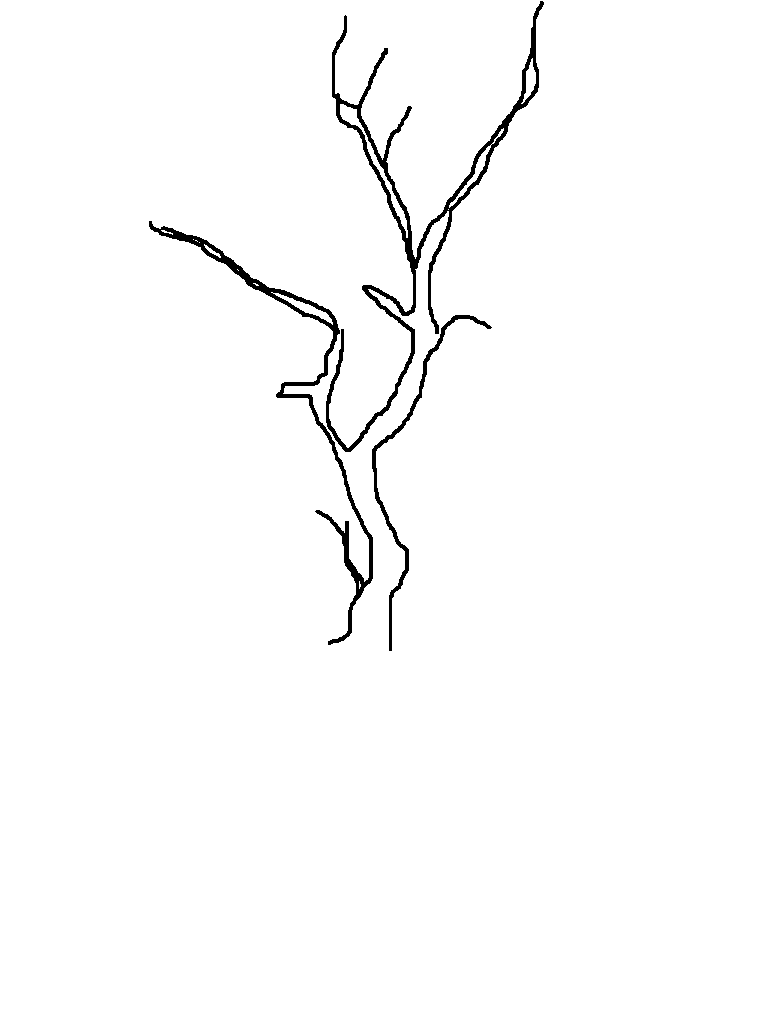
\includegraphics[width=0.3\textwidth,height=2.5cm,keepaspectratio=true]{illustrations/image_examples/sketch_24.png} &
        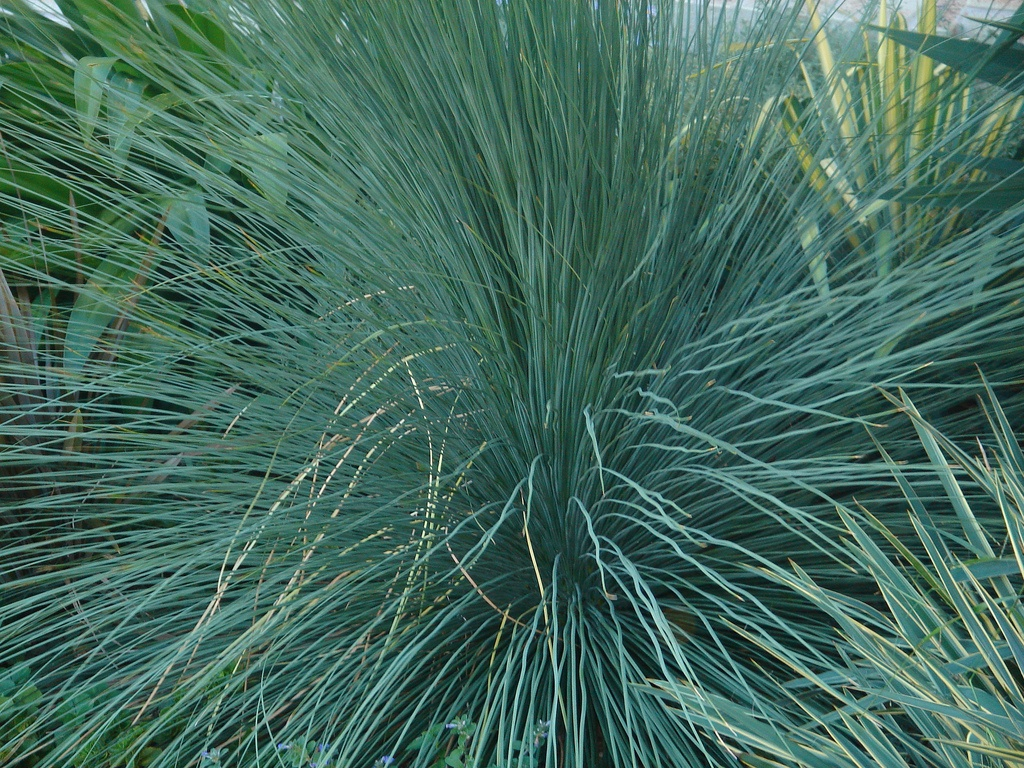
\includegraphics[width=0.3\textwidth,height=2.5cm,keepaspectratio=true]{illustrations/image_examples/result_24_1.jpg} &
        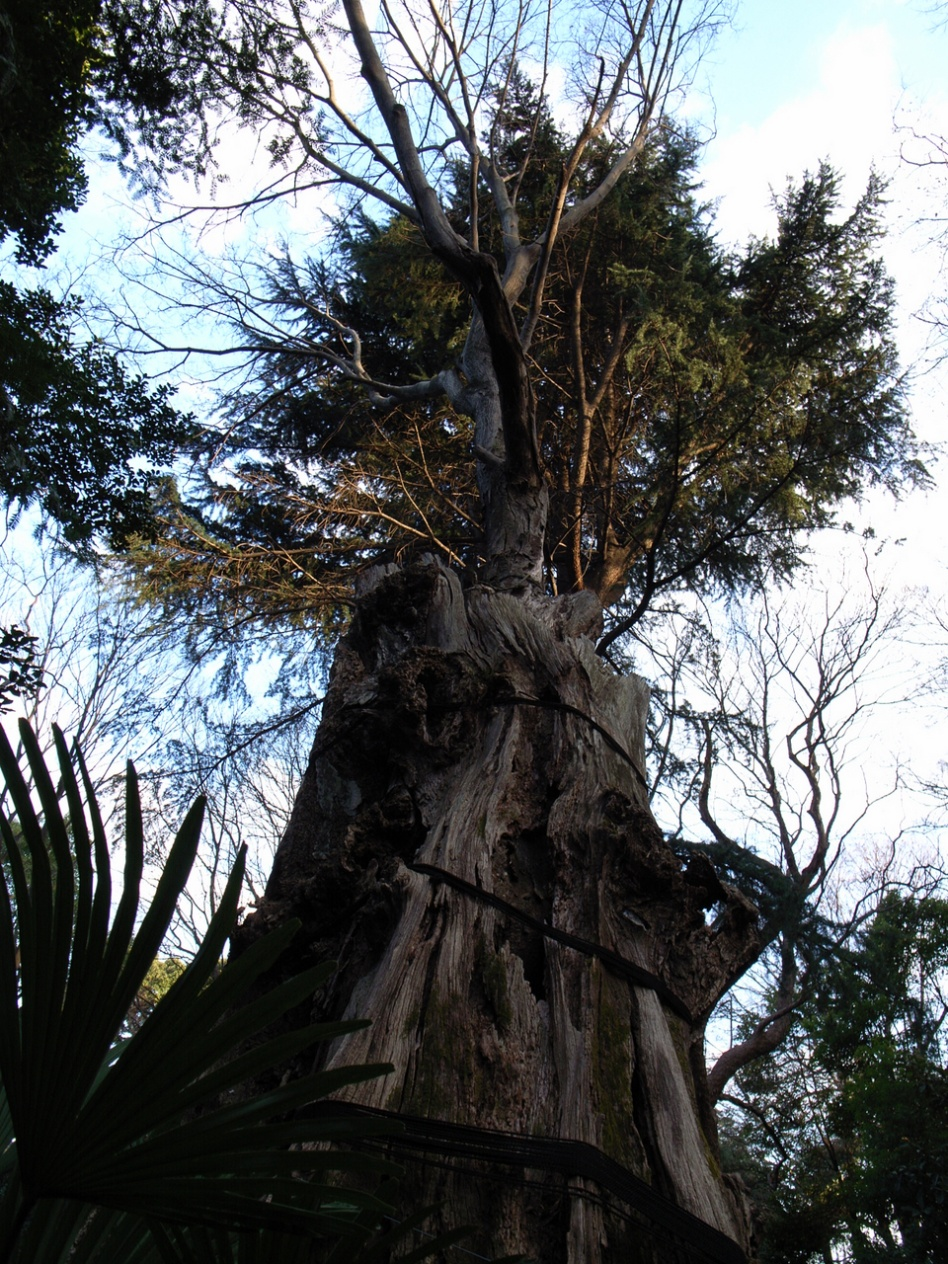
\includegraphics[width=0.3\textwidth,height=2.5cm,keepaspectratio=true]{illustrations/image_examples/result_24_2.jpg} \\
        
\includegraphics[width=0.3\textwidth,height=2.5cm,keepaspectratio=true]{illustrations/image_examples/sketch_42.png} &
        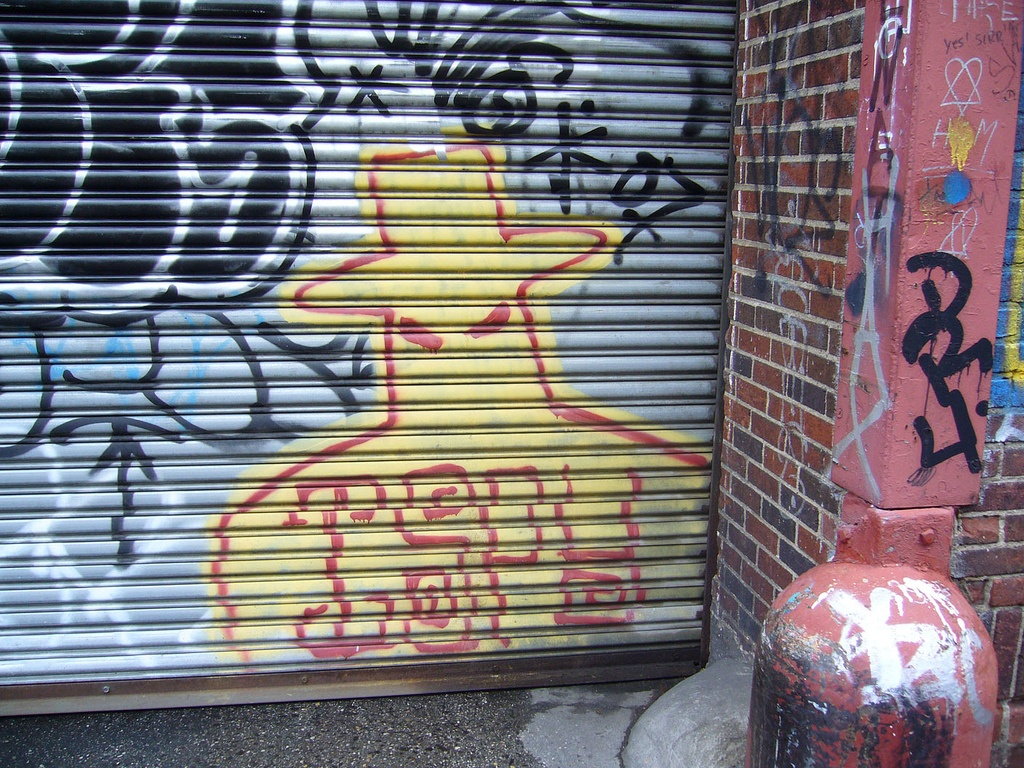
\includegraphics[width=0.3\textwidth,height=2.5cm,keepaspectratio=true]{illustrations/image_examples/result_42_1.jpg} &
        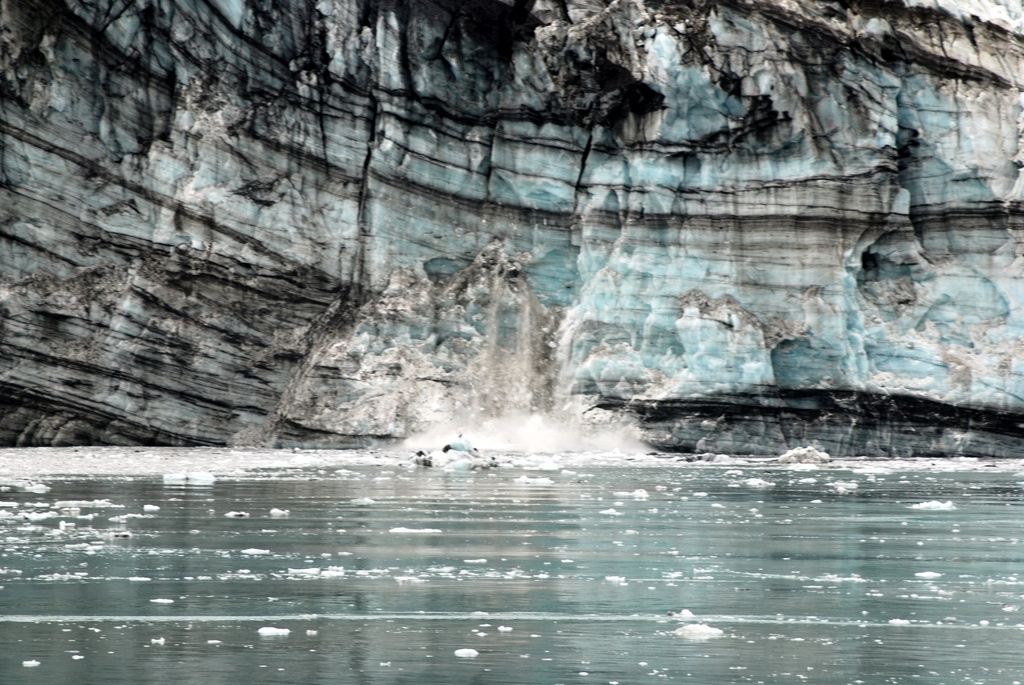
\includegraphics[width=0.3\textwidth,height=2.5cm,keepaspectratio=true]{illustrations/image_examples/result_42_2.jpg}
    \end{tabular}
    \caption[Outlier query images]{
        Outlier query images \texttt{24.png} (top) and \texttt{42.png} (bottom)
        with two example responses.
    }
    \label{fig:results_distribution_outliers}
\end{figure}

\FloatBarrier


